Das Verfahren \glqq Sichtprüfung durch Lichtstreuung\grqq ~wurde in Kapitel \ref{chp:sichtpruefungDurchLichtstreuung} eingeführt und lässt insbesondere kleine Defekte auf spiegelnden Oberflächen sichtbar werden.
%TODO mehr Allgemeines über das Verfahren? -> Ich denke nicht nötig
Die Parameter zur Erzeugung der Muster nach Gleichung \ref{eq:impulsStreifenmuster} können in Tabelle \ref{tab:paramSichtpruefung} abgelesen werden.

\begin{table}[H]
	\centering
	\begin{tabular}{lll}
		\hline 
		\textbf{Beschreibung} & \textbf{Name} & \textbf{Wert} \\ 
		\hline 
		Tastgrad (beeinflusst die Streifenbreiten) & $D$ & $\tfrac{2}{5}$ \\ 
		Amplitude (beeinflusst die Helligkeit) & $A_m$ & 127.5 \\ 
		Kontrast & $C_m$ & 1.0 \\ 
		Anzahl Perioden des Musters & $N_p$ & 128 \\
		Anzahl Phasenverschiebungen & $N_{shift}$ & 16 \\ 
		Bildschirmbreite (in Pixel) & \acrshort{lwidth} & 1920 \\
		Bildschirmhöhe (in Pixel) & \acrshort{lheight} & 1080 \\ 
		\hline 
	\end{tabular}
	\caption{Parameter des Verfahrens}
	\label{tab:paramSichtpruefung}
\end{table}

\noindent
Durch diese Parameter erhält man eine Sequenz aus 16 Mustern die auf einem LCD-Bildschirm angezeigt und anschließend durch eine Kamera aufgenommen werden können.
Zur Kodierung der Oberfläche werden insgesamt 256 Helligkeitsstufen auf die Oberfläche abgebildet.
Zur Verbesserung der Ergebnisse werden die verwendeten Aufbauten durch geeignete Abschirmungen vor Fremdlicht geschützt.

% Durchlichtauswertung
{
	\FloatBarrier
    \subsection{Durchlichtauswertung}
    \label{sub:durchlichtAuswertungLichtstreuung}
    Zunächst wird für dieses Verfahren die Analyse mit der Durchlichtauswertung durchgeführt.
Aus dem Grund werden für die folgenden Bilder nur transparente Brillengläser untersucht.
In Abbildung \ref{tikz:abbStreifenaufnahmen} werden einzelne Aufnahmen der Brillengläser, bei Verwendung des Aufbaus aus dem linken Teilbild aus Abbildung \ref{tikz:abbAufbauFotos}, dargestellt.
Dabei wurden die Brillengläser auf eine dunkle Halterung gelegt, welche im linken Teilbild aus Abbildung \ref{tikz:abbAufbauFotos} über dem Bildschirm zu erkennen ist.

% Abbildung: Streifenaufnahmen
{
	\begin{figure}[H]
		\centering
		\begin{adjustbox}{width=\textwidth}
	\begin{tikzpicture}[every node/.style={inner sep=0,outer sep=0}]
		% Bilder
		\node [anchor=north west] (img1) at (0,0) {\includegraphics[frame,width=.31\textwidth]{05_ergebnisse/ergSichtpruefungDurchLichtstreuung/durchlichtAuswertungLichtstreuung/figures/gefärbtesBrillenglas2_rotiert_Bild}};
		\node [anchor=north west] (img2) at (0.345\textwidth,0) {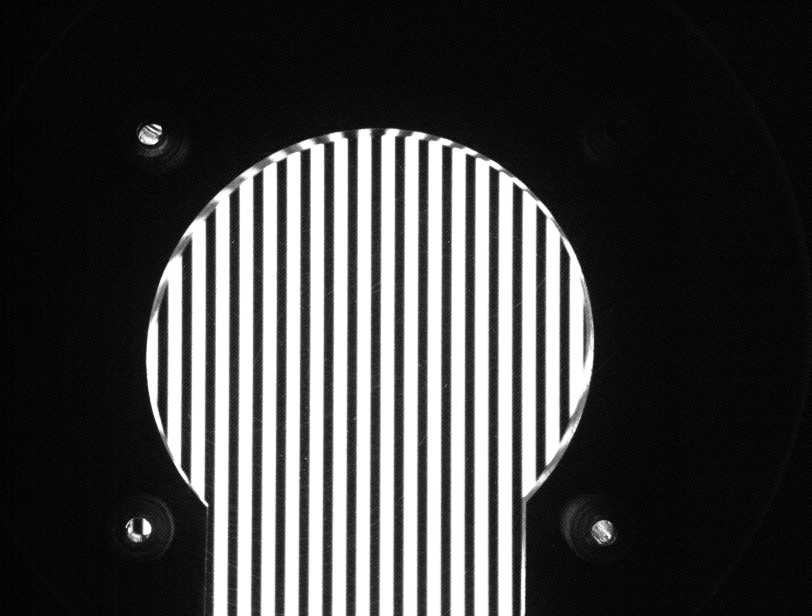
\includegraphics[frame,width=.31\textwidth]{05_ergebnisse/ergSichtpruefungDurchLichtstreuung/durchlichtAuswertungLichtstreuung/figures/polierfehler}};
		\node [anchor=north west] (img3) at (0.69\textwidth,0) {\includegraphics[frame,width=.31\textwidth]{05_ergebnisse/ergSichtpruefungDurchLichtstreuung/durchlichtAuswertungLichtstreuung/figures/HS_Beschädigung}};
		
		% Captions
		\node [below=0.2cm of img1] (cap1) {Brillenglas 1};
		\node [below=0.2cm of img2] (cap2) {Brillenglas 2};
		\node [below=0.2cm of img3] (cap3) {Brillenglas 3};			
	\end{tikzpicture}
\end{adjustbox}
\caption[Aufnahmen der Streifenmuster beim Durchlichtverfahren]{Aufnahmen der Streifenmuster beim Durchlichtverfahren}
		\label{tikz:abbStreifenaufnahmen}
	\end{figure}
}

%TODO Nutzen?
%\noindent
%Das Brillenglas 1 aus Abbildung \ref{tikz:abbStreifenaufnahmen} ist ein polarisierendes Sonnenbrillenglas.
%Das bedeutet, dass die Brille das auftreffende Licht je nach Polarisierung des Lichts deutlich stärker reflektiert.
%Somit gelangt nahezu nur noch Licht in einer speziellen Polarisation durch das Glas.
%Diese Eigenschaft kann man für die Spiegelbildauswertung nutzen um den Rückseitenreflex (vgl. Abschnitt \ref{sec:spiegelndeOberflaechen}) zu minimieren.

\noindent
Durch Anwendung des Verfahrens \glqq Sichtprüfung durch Lichtstreuung\grqq erhält man für die drei Brillengläser folgende Bilder:

% Abbildung: Ergebnis der Sichtprüfung durch Lichtstreuung
{
	\begin{figure}[H]
		\centering
		\begin{adjustbox}{width=\textwidth}
	\begin{tikzpicture}[every node/.style={inner sep=0,outer sep=0}]
		% Bilder
		\node [anchor=north west] (img1) at (0,0) {\includegraphics[frame,width=.31\textwidth]{05_ergebnisse/ergSichtpruefungDurchLichtstreuung/durchlichtAuswertungLichtstreuung/figures/gefärbtesBrillenglas2_rotiert_sichtpruefungLichtstreuung}};
		\node [anchor=north west] (img2) at (0.345\textwidth,0) {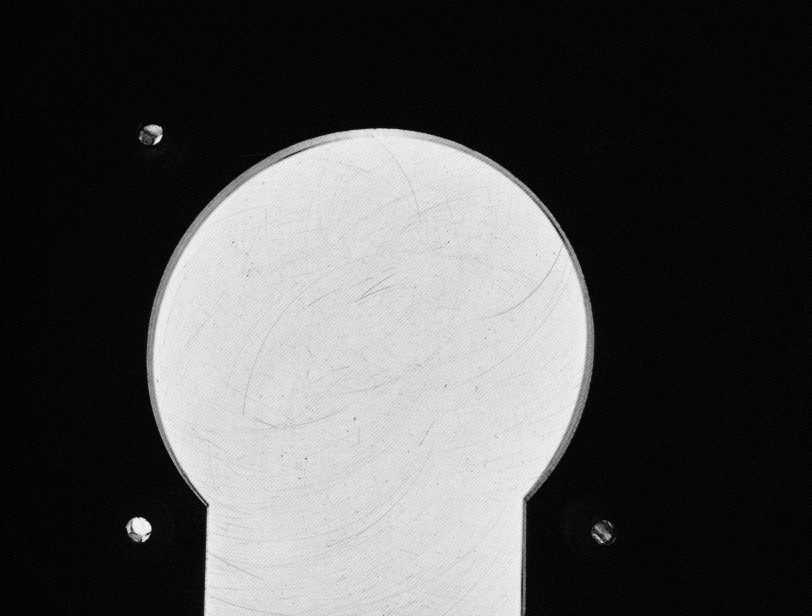
\includegraphics[frame,width=.31\textwidth]{05_ergebnisse/ergSichtpruefungDurchLichtstreuung/durchlichtAuswertungLichtstreuung/figures/polierfehler_ergebnis}};
		\node [anchor=north west] (img3) at (0.69\textwidth,0) {\includegraphics[frame,width=.31\textwidth]{05_ergebnisse/ergSichtpruefungDurchLichtstreuung/durchlichtAuswertungLichtstreuung/figures/HS_Beschädigung_ergebnis}};
		
		% Captions
		\node [below=0.2cm of img1] (cap1) {Brillenglas 1};
		\node [below=0.2cm of img2] (cap2) {Brillenglas 2};
		\node [below=0.2cm of img3] (cap3) {Brillenglas 3};			
	\end{tikzpicture}
\end{adjustbox}
\caption[Ergebnisbilder des Verfahrens \glqq Sichtprüfung durch Lichtstreuung\grqq]{Ergebnisbilder des Verfahrens \glqq Sichtprüfung durch Lichtstreuung\grqq}
		\label{tikz:abbCombinePatternPictures}
	\end{figure}
}

\noindent
Um die Bilder aus Abbildung \ref{tikz:abbCombinePatternPictures} zu erzeugen wurde als Verknüpfungsmethode des  Verfahrens die betragsmäßige Differenz gewählt, um einen hohen Kontrast zwischen der Halterung und dem sichtbaren Bereich des Brillenglases zu erzeugen.
Durch Anwendung einer Kontrastverbesserung in lokalen Bereichen des Bildes und geeigneter Kennlinientransformationen können die Bilder nachbearbeitet werden, um die Kratzer und Eingravierungen in der Oberfläche besser zu erkennen:

% Abbildung: Nachbearbeitung der Ergebnisbilder
{
	\begin{figure}[H]
		\centering
		\begin{adjustbox}{width=\textwidth}
	\begin{tikzpicture}[every node/.style={inner sep=0,outer sep=0}]
		% Bilder
		\node [anchor=north west] (img1) at (0,0) {\includegraphics[width=.31\textwidth]{05_ergebnisse/ergSichtpruefungDurchLichtstreuung/durchlichtAuswertungLichtstreuung/figures/gefärbtesBrillenglas2_rotiert_verbessert_Norm_LookUp}};
		\node [anchor=north west] (img2) at (0.345\textwidth,0) {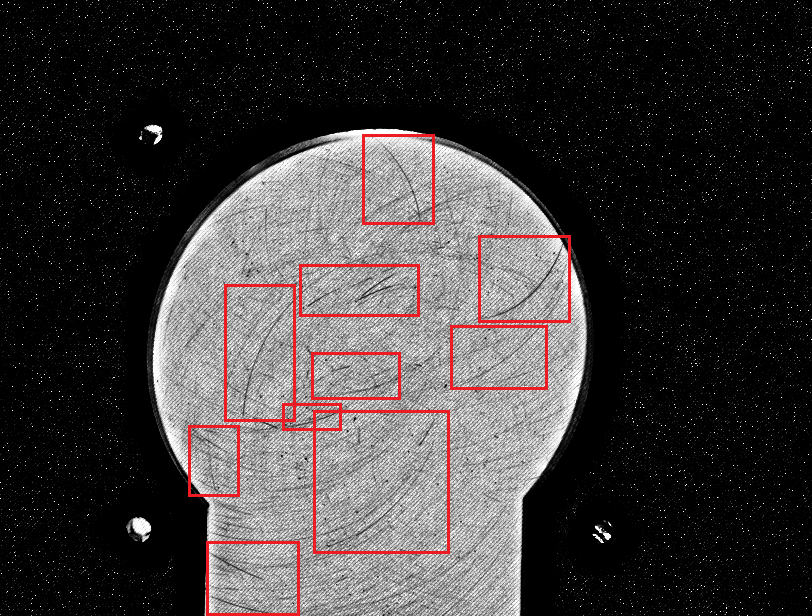
\includegraphics[width=.31\textwidth]{05_ergebnisse/ergSichtpruefungDurchLichtstreuung/durchlichtAuswertungLichtstreuung/figures/polierfehler_ergebnis_verbessert}};
		\node [anchor=north west] (img3) at (0.69\textwidth,0) {\includegraphics[width=.31\textwidth]{05_ergebnisse/ergSichtpruefungDurchLichtstreuung/durchlichtAuswertungLichtstreuung/figures/HS_Beschädigung_ergebnis_verbessert}};
		
		% Captions
		\node [below=0.2cm of img1] (cap1) {Brillenglas 1};
		\node [below=0.2cm of img2] (cap2) {Brillenglas 2};
		\node [below=0.2cm of img3] (cap3) {Brillenglas 3};			
	\end{tikzpicture}
\end{adjustbox}
\caption[Verbesserung der Ergebnisbilder]{Verbesserung der Ergebnisbilder. In Grün: Gravur der Brillenglaskennzeichnung. In Rot: Kratzer und ähnliche Beschädigungen der Oberfläche.\footnotemark}
		\label{tikz:abbNachbearbeitung}
	\end{figure}
	\footnotetext{Es wurde nur eine Auswahl von Fehlstellen markiert, um die Übersicht beizubehalten.}
}

\noindent
In den einzelnen Teilbildern aus Abbildung \ref{tikz:abbNachbearbeitung} kann man in den markierten Bereichen Fehlstellen bzw. Gravuren als dunkle Formen erkennen.
}

% Spiegelbildauswertung
{
	\FloatBarrier
    \subsection{Spiegelbildauswertung}
    \label{sub:spiegelbildAuswertungLichtstreuung}
    Nachdem das Verfahren für die Durchlichtauswertung Fehlstellen auf transparenten Objekten sichtbar machen konnte, stellt man sich die Frage, ob ähnliche Ergebnisse auch für nicht-transparente spiegelnde Objekte erzielt werden können.
Für diese Objekte wird das Verfahren mit der Spiegelbildauswertung durchgeführt.
Hierfür wählt man den Aufbau aus dem rechten Teilbild aus Abbildung \ref{tikz:abbAufbauFotos}.

\p
Für einen Vergleich der Spiegelbildauswertung zur Durchlichtauswertung für transparente Prüfobjekte wird das Brillenglas 1 (siehe linkes Teilbild aus Abbildung \ref{tikz:abbStreifenaufnahmen}) gewählt, da es durch ein polarisierendes Sonnenbrillenglas ist.
Das bedeutet, dass das Brillenglas das auftreffende Licht je nach Polarisierung des Lichts deutlich stärker reflektiert.
Somit gelangt nahezu nur noch Licht mit einer speziellen Polarisation durch das Glas.
Diese Eigenschaft kann man für die Spiegelbildauswertung nutzen um den Rückseitenreflex (vgl. Abschnitt \ref{sec:spiegelndeOberflaechen}) zu minimieren.
Die weiteren Objekte sind spiegelnde Keramikbruchstücke.

% Abbildung: Streifenaufnahmen
{
	\begin{figure}[H]
		\centering
		\begin{adjustbox}{width=\textwidth}
	\begin{tikzpicture}[every node/.style={inner sep=0,outer sep=0}]
		% Bilder
		\node [anchor=north west] (img1) at (0,0) {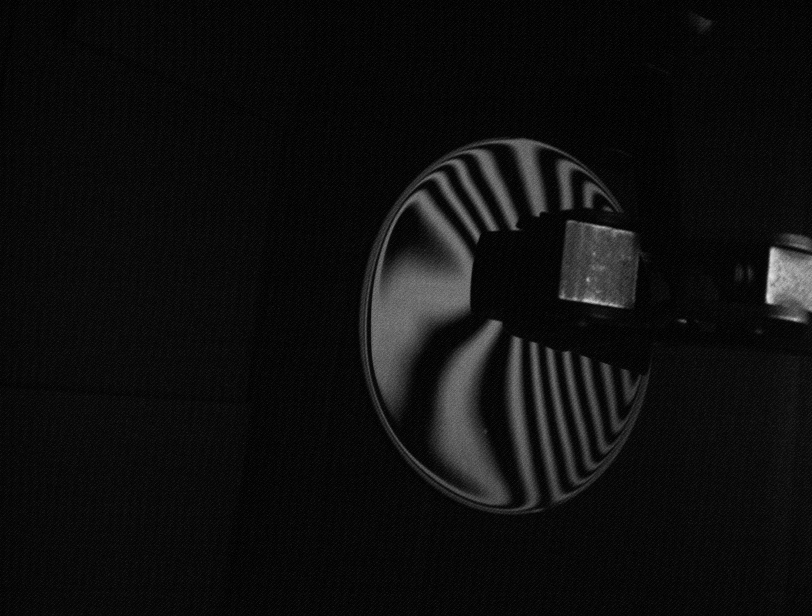
\includegraphics[width=.31\textwidth]{05_ergebnisse/ergSichtpruefungDurchLichtstreuung/spiegelbildAuswertungLichtstreuung/figures/brillenglas_1_beleuchtetImpuls}};
		\node [anchor=north west] (img2) at (0.345\textwidth,0) {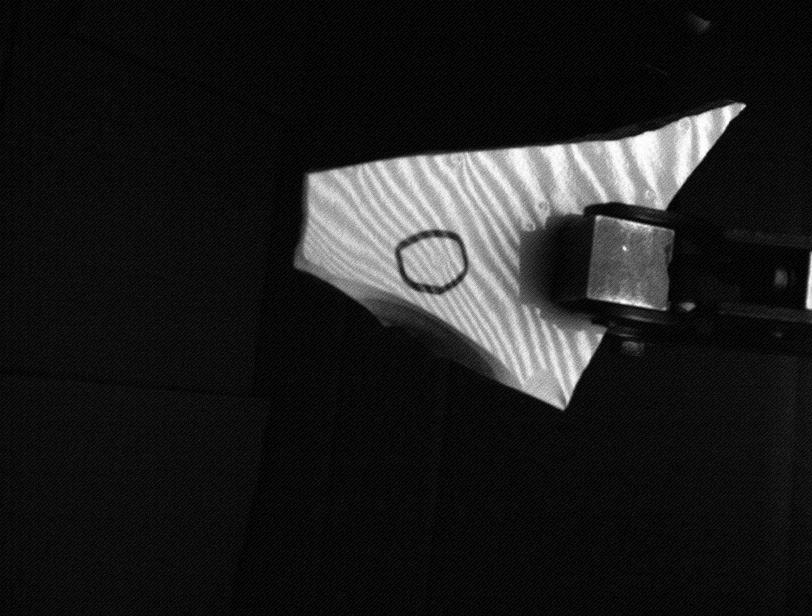
\includegraphics[width=.31\textwidth]{05_ergebnisse/ergSichtpruefungDurchLichtstreuung/spiegelbildAuswertungLichtstreuung/figures/keramikObjekt_1_beleuchtetImpuls}};
		\node [anchor=north west] (img3) at (0.69\textwidth,0) {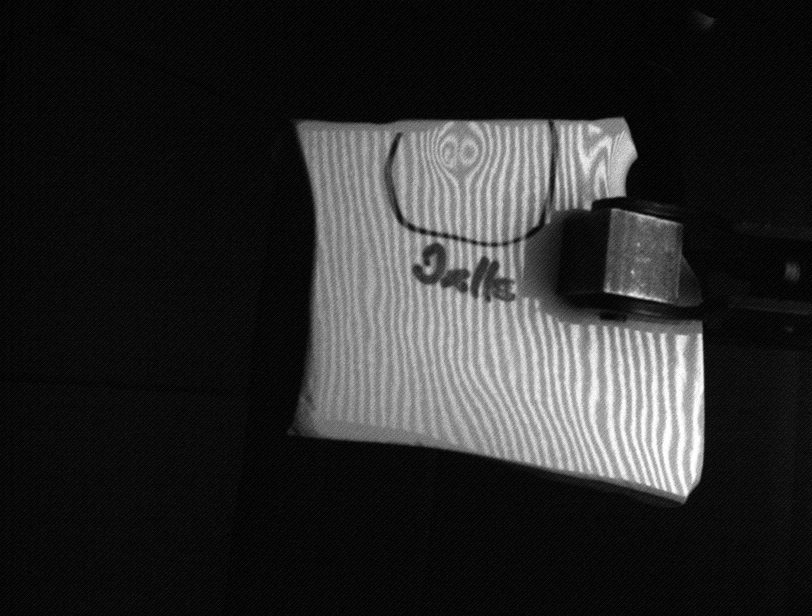
\includegraphics[width=.31\textwidth]{05_ergebnisse/ergSichtpruefungDurchLichtstreuung/spiegelbildAuswertungLichtstreuung/figures/keramikObjekt_2_beleuchtetImpuls}};
		
		% Captions
		\node [below=0.2cm of img1] (cap1) {Brillenglas 1};
		\node [below=0.2cm of img2] (cap2) {Keramikobjekt 1};
		\node [below=0.2cm of img3] (cap3) {Keramikobjekt 2};			
	\end{tikzpicture}
\end{adjustbox}
\caption[Aufnahmen der Streifenmuster bei der Spiegelbildauswertung]{Aufnahmen der Streifenmuster bei der Spiegelbildauswertung}
		\label{tikz:abbStreifenaufnahmenSpLichtstreuung}
	\end{figure}
}

\noindent
Durch Anwendung des Verfahrens \glqq Sichtprüfung durch Lichtstreuung\grqq ~erhält man für die drei Prüfobjekte folgende Bilder:

% Abbildung: Ergebnis der Sichtprüfung durch Lichtstreuung
{
	\begin{figure}[H]
		\centering
		\begin{adjustbox}{width=\textwidth}
	\begin{tikzpicture}[every node/.style={inner sep=0,outer sep=0}]
		% Bilder
		\node [anchor=north west] (img1) at (0,0) {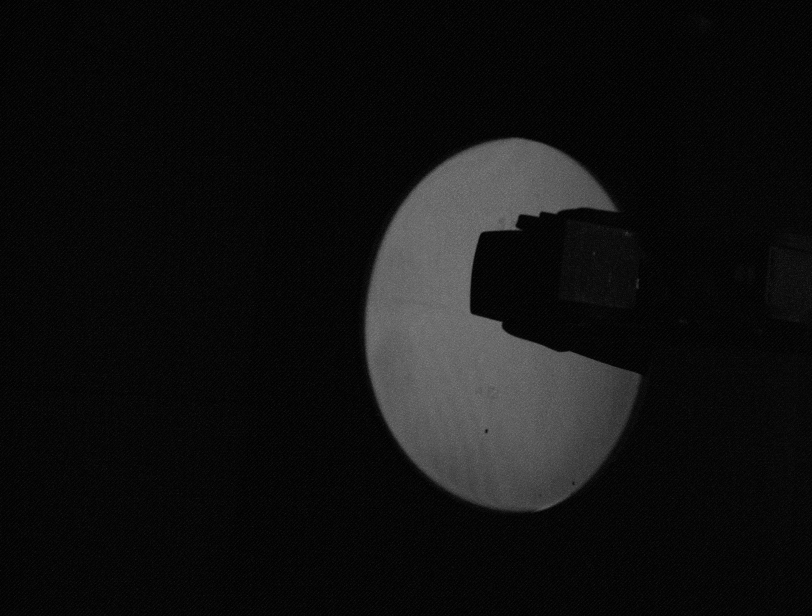
\includegraphics[width=.31\textwidth]{05_ergebnisse/ergSichtpruefungDurchLichtstreuung/spiegelbildAuswertungLichtstreuung/figures/brillenglas_1_combinePattern}};
		\node [anchor=north west] (img2) at (0.345\textwidth,0) {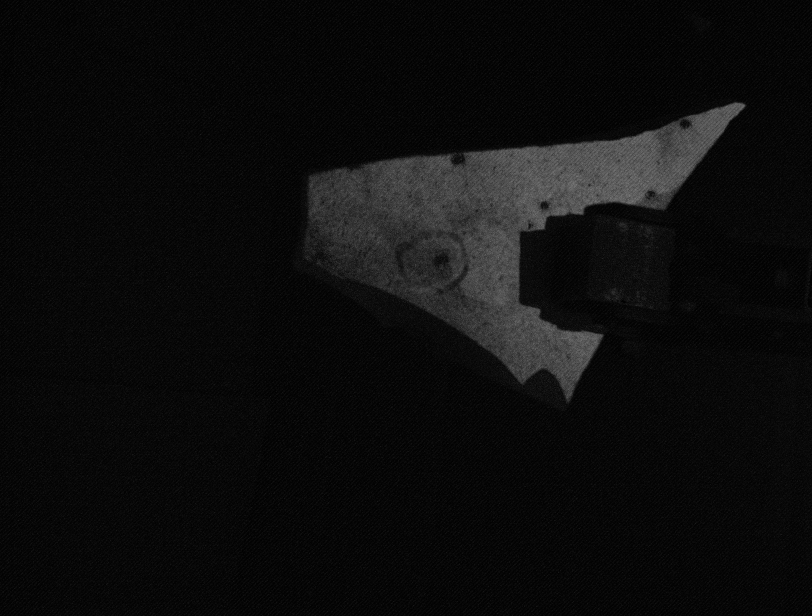
\includegraphics[width=.31\textwidth]{05_ergebnisse/ergSichtpruefungDurchLichtstreuung/spiegelbildAuswertungLichtstreuung/figures/keramikObjekt_1_combinePattern}};
		\node [anchor=north west] (img3) at (0.69\textwidth,0) {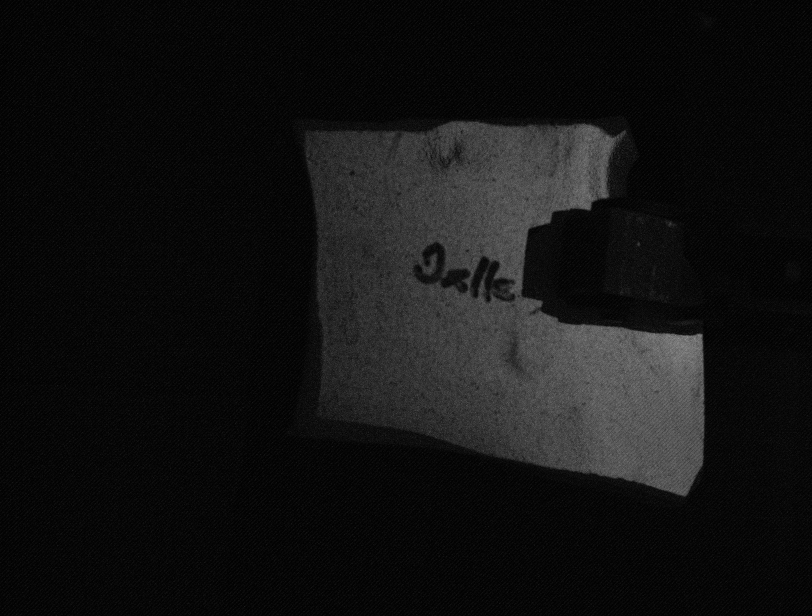
\includegraphics[width=.31\textwidth]{05_ergebnisse/ergSichtpruefungDurchLichtstreuung/spiegelbildAuswertungLichtstreuung/figures/keramikObjekt_2_combinePattern}};
		
		% Captions
		\node [below=0.2cm of img1] (cap1) {Brillenglas 1};
		\node [below=0.2cm of img2] (cap2) {Keramikobjekt 1};
		\node [below=0.2cm of img3] (cap3) {Keramikobjekt 2};		
	\end{tikzpicture}
\end{adjustbox}
\caption[Ergebnisbilder des Verfahrens \glqq Sichtprüfung durch Lichtstreuung\grqq ~bei der Spiegelbildauswertung]{Ergebnisbilder des Verfahrens \glqq Sichtprüfung durch Lichtstreuung\grqq ~bei der Spiegelbildauswertung}
		\label{tikz:abbCombinePatternPicturesSpLichtstreuung}
	\end{figure}
}

\noindent
Es wurde als Verknüpfungsmethode des Verfahrens die betragsmäßige Differenz gewählt, um die Bilder aus Abbildung \ref{tikz:abbCombinePatternPicturesSpLichtstreuung} zu erzeugen.
Auch hier ist die Begründung der höhere Kontrast zwischen den Prüfobjekten und dem Hintergrund.
In einem weiterem Schritt wurden die Bilder durch lokale Kontrastverbesserungen und geeigneter Kennlinientransformationen nachbearbeitet, um die Fehlstellen besser zu erkennen:

% Abbildung: Nachbearbeitung der Ergebnisbilder
{
	\begin{figure}[H]
		\centering
		\begin{adjustbox}{width=\textwidth}
	\begin{tikzpicture}[every node/.style={inner sep=0,outer sep=0}]
		% Bilder
		\node [anchor=north west] (img1) at (0,0) {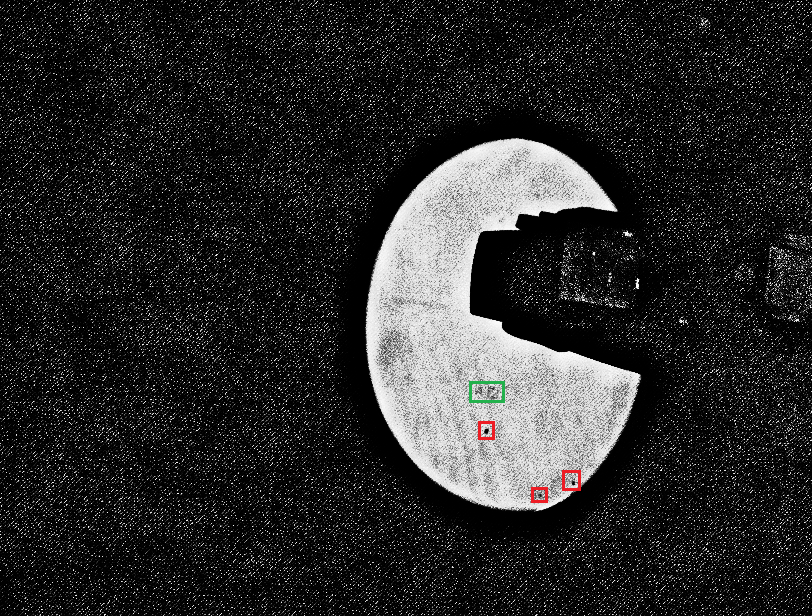
\includegraphics[width=.31\textwidth]{05_ergebnisse/ergSichtpruefungDurchLichtstreuung/spiegelbildAuswertungLichtstreuung/figures/brillenglas_1_verbessert}};
		\node [anchor=north west] (img2) at (0.345\textwidth,0) {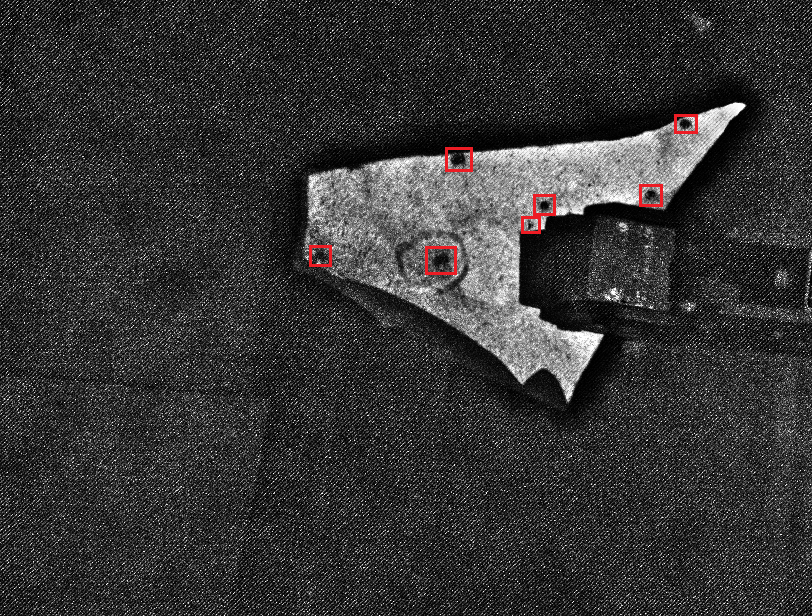
\includegraphics[width=.31\textwidth]{05_ergebnisse/ergSichtpruefungDurchLichtstreuung/spiegelbildAuswertungLichtstreuung/figures/keramikObjekt_1_verbessert}};
		\node [anchor=north west] (img3) at (0.69\textwidth,0) {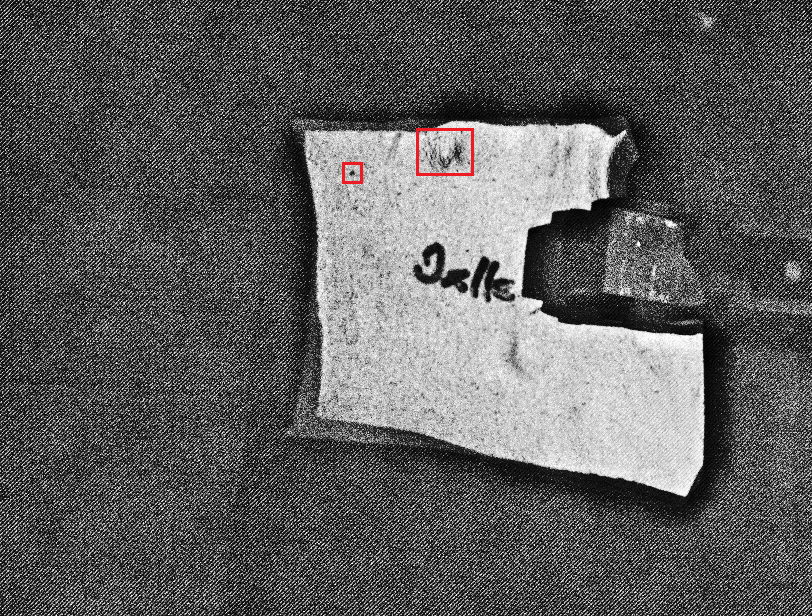
\includegraphics[width=.31\textwidth]{05_ergebnisse/ergSichtpruefungDurchLichtstreuung/spiegelbildAuswertungLichtstreuung/figures/keramikObjekt_2_verbessert}};
		
		% Captions
		\node [below=0.2cm of img1] (cap1) {Brillenglas 1};
		\node [below=0.2cm of img2] (cap2) {Keramikobjekt 1};
		\node [below=0.2cm of img3] (cap3) {Keramikobjekt 2};
	\end{tikzpicture}
\end{adjustbox}
\caption[Verbesserung der Ergebnisbilder]{Verbesserung der Ergebnisbilder. In Grün (bei Brillenglas 1): Gravur der Brillenglaskennzeichnung. In Rot: Kratzer, Pickel und ähnliche Be\-schä\-di\-gun\-gen der Oberfläche.}
		\label{tikz:abbNachbearbeitungSpLichtstreuung}
	\end{figure}
}

\noindent
In Abbildung \ref{tikz:abbNachbearbeitungSpLichtstreuung} sind die Fehlstellen in Rot markiert. 
Analog wie auch im vorherigen Abschnitt \ref{sub:durchlichtAuswertungLichtstreuung} erkennt man für Brillenglas 1 im grünen Rechteck eine Gravur des Markenzeichens auf der Oberfläche.
Für das Keramikobjekt 1 fallen einige dunkle Punkte im Objektbereich auf, welche durch sogenannte \glqq Pickel \grqq ~auf der Oberfläche entstehen.
Auf dem Keramikobjekt 2 befindet sich eine Delle, die im größeren roten Rechteck zu sehen ist.

%TODO Abschluss der Section?
}